\clearpage
\section{Results}
We present the results of our empirical analysis for the sample of experts (the WES sample) and the sample of non-experts (the prolific sample).  We estimate the following model using binary logit. 
\begin{equation*}
    Y_{ijc}= \alpha_{j}+ \beta *D_{c} + \gamma*X_{i}
\end{equation*}
Where $Y_{ijc}$ denotes the response of individual $i$ from country $c$ to question $j$ we will control for individual characteristics $X_{i}$ such as age, level of education, gender and employment status (affiliation for the expert sample). The dummy variable $D_{c}$ indicates whether the expert's nationality is Greek, Cypriotic, Spanish, Irish or Portuguese with the coefficient $\beta$ measuring the divergence in the answers of participants from program and non-program countries. \footnote{In the expert sample participants are asked in which country they were born}For questions in which participants were asked to state their level of agreement we estimate the effect of being from a program country on the likelihood to strongly or slightly agree. For questions in which participants are asked to name the responsible party, we estimate the effect of being from a program country on the likelihood to state "Lender countries". \\ \\
\textbf{Baseline Results} 
When asked about the intentions of lender countries to initiate the credit relationship our hypothesis is verified among our non-expert participants.
 In the non-expert sample citizens from program countries are 10.9 percentage points more likely to agree that lender countries wanted to impose institutional change upon the borrower countries. They are 13.1 percentage points less likely to agree that the lender countries wanted to help the borrowing countries. However, there is no significant effect on agreeing that lender countries merely wanted to avoid a crisis at home. In the expert sample there are no statistically significant differences in the assessments of experts from program and non-program countries. Contrasting our hypothesis,  experts from program countries are more likely to agree that the lender countries wanted to help the borrowing countries. This effect does not turn out to be statistically significant.  \\ 
 \begin{figure}[H]
\begin{center}
     \caption{ Hypothesis 1: Why the lender countries initiated the credit relationship}
    
     \includegraphics[scale=0.8]{Question2_base.pdf}
     \label{fig:my_label}
      \end{center}
      \tiny
     \tablenotes{The sign in parantheses denotes the predicted differential effect. Participants were asked to assess the following statements:  Question 2.1: The lender countries wanted to help the borrowing countries Question 2.2: The lender countries wanted to help themselves avoid a crisis at home Question 2.3: The lender countries wanted to impose institutional change upon the borrower countries  }
\end{figure}
 We continue to ask the participants about the emotions the rescue program evoked among citizens from the borrower and lender countries. The hypothesis that lenders have a blind spot regarding the feelings of citizens from borrower countries is confirmed. Participants from program countries in the non-expert sample are 9.2 and 9.3 percentage points more likely to agree that the rescue experience made them feel guilty and inferior. Further, the probability to agree to "The rescue experience made many citizens in the borrower countries feel exploited" increases by 16.9 percentage points among citizens from program countries. All effects are statistically significant at the 1 percent level. Among the sample of economic experts the effect sizes are smaller and not significantly different from zero. \\
 Interestingly, we do not find that borrowers have a blind spot regarding the emotions the program evoked among lender countries. There are only small differences in the likelihood to agree with certain statements between citizens from program and non-program countries which are not significant. There is no difference in evaluating the effect of the rescue program on the friendship between citizens. The results are similar in the expert and non-expert sample. \\

 We further predicted that borrower countries will be more confident that they will be able to repay outstanding debt. 
 When asked whether Greece \footnote{We only ask about Greece, since Greece remains the only country that has not repaid it's debt} will be capable of fully paying back it's debt, citizens from program countries show a 13.5 percentage point higher likelihood to agree in the non-expert sample and a 12.2 percentage point higher likelihood in the expert sample. This effect is again significant at the 1 percent level. \\
 \begin{figure} [h!]
    \begin{center}
    \caption{Hypothesis 4: Feelings evoked among citizens from program countries}
    \includegraphics[scale=0.8]{Question5_1_base.pdf}
    \label{fig:my_label}
    \end{center}
    \tiny
    \tablenotes{The sign in parantheses denotes the predicted differential effect. Question 5.1: The rescue experience made many citizens in the borrower countries feel guilty; Question 5.2: The rescue experience made many citizens in the borrower countries feel exploited; Question 5.3: The rescue experience made many citizens in the borrower countries feel inferior. }
\end{figure}
\begin{figure}[h!]
\begin{center}
\caption{Hypothesis 4 and 5: Feelings evoked among citizens from non-program countries }

    \includegraphics[scale=0.8]{Question5_2_base.pdf}
    \label{fig:my_label}
    \end{center}
    \tiny
    \tablenotes{The sign in parantheses denoted the predicted differential effect. Question 5.4: The rescue experience made many citizens in the lender countries feel exploited; Question 5.5 The rescue experience made many citizens in the lender countries feel disappointed Question 5.6: The rescue experience strengthened friendships between citizens Question 7: Greece will fully pay back it's debt}
\end{figure}
 
%  \begin{figure}
%\caption{Assessment of the emotions the program evoked among different parties}
%\centering
%\begin{minipage}{.5\textwidth}
% \includegraphics[scale=0.5]{Question5_1_base.pdf}
 %\end{minipage}%
 %\hfill
%\begin{minipage}{.5\textwidth}
%\includegraphics[scale=0.5]{Question5_2_base.pdf}
%\end{minipage}
%\end{figure}
 We proceed to evaluate who initiated and who benefited from the credit relationship. 
In the non-expert sample citizens are 13.2 percentage points more likely to state that the lender countries were the driving force behind signing the memorandum. Further, they are 28 percentage points more likely to state that the lender countries were the main beneficiaries of the program and 20.3 percentage points more likely to state that lender countries benefited from the loans to Greece. All effects are statistically significant at the one percent level. We do not find statistically significant effects in the expert sample. Interestingly, the mean difference between expert and non-experts is negative, contrary to the anticipated effect. Experts from program countries are for example 12.4 percentage points less likely to state that citizens from lender countries were the main beneficiary from the program.\\
\begin{figure}[h!] 
\begin{center}
     \caption{Hypothesis 2 and 3: Who initiated and benefited from the rescue program}
     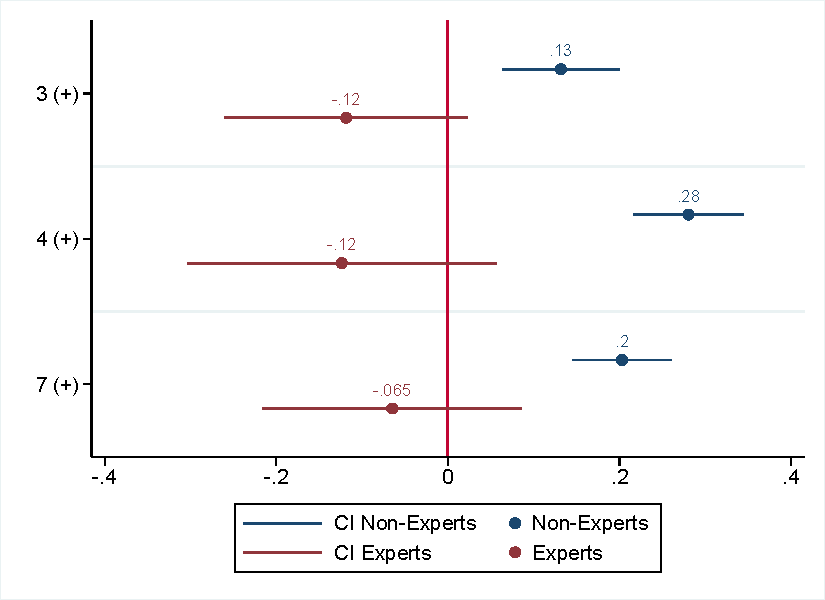
\includegraphics[scale=0.8]{Question3_base.pdf}
     \label{fig:my_label}
     \end{center}
     \tiny
     \tablenotes{The sign in parantheses denotes the predicted differential effect.Question 3: Who was the driving force behind signing the memorandum; Question 4: Who was the main beneficiary of the program; Question 7: Who primarily benefited from the loans to Greece}
\end{figure}

\textbf{Sample Splits}
Program and non-program countries vary along other dimensions than the program and non-program distinction. Program countries have some common characteristics that are likely to influence the estimates. Hence, we conduct sample splits along different macroeconomic variables to assess whether these macroeconomic characteristics influence the magnitude of our effect. Countries which were affected by the European debt crisis are predominantly Southern European and are located at the periphery of the European Union (measured by distance to Brussels). Further, all these countries experienced a substantial increase in debt levels, high levels of unemployment and low GDP growth. We also estimate our model on the subsample of all countries in the Eurozone. In the non-expert sample there are few changes to the baseline results, when splitting the sample along these different characteristics. When asked about the intentions behind entering the rescue program the findings from the baseline regression persist among all sample splits. The effect in the sample of countries with high levels of unemployment becomes smaller and is only significant at the five percent level. In the sample of southern European countries the disagreement over whether lender countries wanted to impose institutional change on borrower countries also decreases and is only significant at the five percent level. Interestingly, the estimates for the sample of periphery countries are much larger than in the baseline sample. In the periphery sample participants from program countries are 19.1 percentage points less likely to agree with the statement that the lender countries wanted to help the borrowing countries and 14.2 percentage points more likely to agree that lender countries wanted to impose institutional change compared to respectively 13.1 and 11.1 percentage points in the full sample.\\
When asked about the emotions of citizens in borrower and lender countries the estimates become slightly smaller in the southern European, periphery and high debt sample than for the full sample. The divergence in assessments about whether the rescue program made the citizens in the borrower countries feel inferior even becomes insignificant in the Southern European sample. Among all samples there is substantial disagreement between program and non-program countries that Greece will repay it's debt. 
\\
The magnitude and significance levels of effects of the program variable remains relatively unchanged for the remainder of questions. There are no differences in the effects of the full sample and all subsamples when asked about the driving force behind the referendum. Further, there is no difference in effects across samples when asked about the main beneficiary of the program. A detailed overview of the results across all sample splits is included in the appendix. 